\documentclass[border=3pt,tikz]{standalone}
\usepackage{amsmath}
\usetikzlibrary{calc}
\usetikzlibrary{arrows.meta} % for arrow size
\usetikzlibrary{calc,patterns,angles,quotes}
\begin{document}

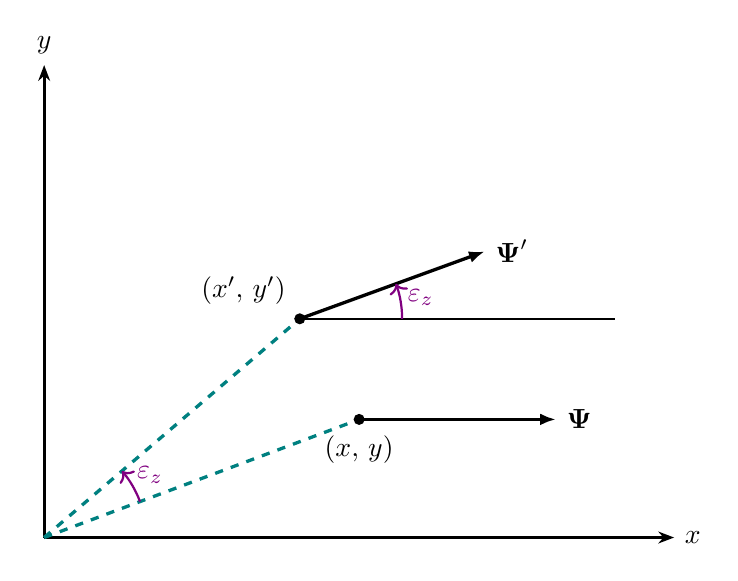
\begin{tikzpicture}[scale=1]
    \usetikzlibrary {arrows.meta}
    \usetikzlibrary {calc}
    
    \draw[very thick, -{Stealth[length=2mm]}] (0, 0) -- (8, 0) node [right] {$x$} ;
    \draw[very thick, -{Stealth[length=2mm]}] (0, 0) -- (0, 6) node [above] {$y$};
    
    \def\x1{4};
    \def\y1{1.5};
    \def\th{20}
    \def\c{2.5}
    \coordinate (O) at (0, 0);
    \coordinate (A) at (\x1, \y1);
    \coordinate (B) at ({\x1*cos(\th) -\y1*sin(\th)}, {\x1*sin(\th) + \y1*cos(\th)});
    \coordinate (C) at (\c, 0);
    \coordinate (D) at ({\c*cos(\th)}, {\c*sin(\th)});
    \coordinate (AC) at ($(A) + (C)$);
    \coordinate (BD) at ($(B) + (D)$);
    \coordinate (BB) at ($(B) + (4, 0)$);
    \draw[very thick, teal, dashed] (O) -- (A);
    \draw[very thick, teal, dashed] (O) -- (B);
    \node[circle,fill=black,inner sep=0pt,minimum size=4pt,label=below:{$(x,\,y)$}] at (A) {};
    \node[circle,fill=black,inner sep=0pt,minimum size=4pt,label=above left:{$(x',\,y')$}] at (B) {};
    \draw[very thick, -{Latex[length=2mm]}] (A) -- (AC) node [right] {$\boldsymbol{\Psi}$};
    \draw[very thick, -{Latex[length=2mm]}] (B) -- (BD) node [right] {$\boldsymbol{\Psi}'$};
    \draw[thick, ] (B) -- (BB) ;
    \pic [draw, thick, violet, angle radius=1.3cm, ->, "$\varepsilon_z$",  angle eccentricity=1.2] {angle = A--O--B};
    \pic [draw, thick, violet, angle radius=1.3cm, ->, "$\varepsilon_z$",  angle eccentricity=1.2] {angle = BB--B--BD};

    \end{tikzpicture}
    \end{document}